\documentclass[ dottedtoc,oneside,openright,titlepage,numbers=noenddot,headinclude,letterpaper
                footinclude=true,cleardoublepage=empty,abstractoff,
                paper=letterpaper,fontsize=12pt,
                ngerman,american,
                ]{scrreprt}

%********************************************************************
% Note: Make all your adjustments in here
%*******************************************************
% \usepackage{algorithm}% http://ctan.org/pkg/algorithms
\usepackage{algorithm2e}
% \usepackage{algpseudocode}% http://ctan.org/pkg/algorithmicx

\usepackage{comment}
\usepackage{adjustbox}
\usepackage[section]{placeins}
\usepackage{listings}
\usepackage{longtable}
\usepackage{colortbl}
\usepackage{caption}
\usepackage{setspace}
% *****************************************************************************
% Triggers for this config
% *****************************************************************************
\usepackage{ifthen}
\newboolean{enable-backrefs} % enable backrefs in the bibliography
\setboolean{enable-backrefs}{false} % true false
% *****************************************************************************


% *****************************************************************************
% 2. Personal data and user ad-hoc commands
% *****************************************************************************
\newcommand{\invpyr}[1]{\vbox{\hsize=4.5in \parindent=0pt \emergencystretch=1in
  \parshape 6
    0.00in 4.50in
    0.25in 4.00in
    0.50in 3.50in
    0.75in 3.00in
    1.00in 2.50in
    1.25in 2.00in
    \leftskip=0pt plus 1fil \rightskip=0pt plus -1fil
    \parfillskip=0pt plus 2fil
    #1}}


\newcommand{\myTitle}{Optimizing Energy Consumption of Edge IoT Devices \xspace}
\newcommand{\myTITLE}{\expandafter\MakeUppercase\expandafter{\myTitle}}


\newcommand{\mySubtitle}{\singlespacing A thesis submitted to the Graduate
College of \\ 
Texas State University in partial fulfillment \\
of the requirements for the degree of\\}
\newcommand{\myDegree}{Master of Science \\ with a Major in Computer Science\xspace}


\newcommand{\myName}{Mujahid Khan\xspace}
\newcommand{\myProf}{Dr. Anne Hee Hiong Ngu\xspace}
\newcommand{\myOtherProf}{Put name here\xspace}
\newcommand{\mySupervisor}{You Advisor\xspace}
\newcommand{\myFaculty}{Put data here\xspace}
\newcommand{\myDepartment}{Department of Computer Science\xspace}
\newcommand{\myUni}{Texas State University\xspace}
\newcommand{\myLocation}{San Marcos\xspace}
\newcommand{\myTime}{December 2021\xspace}  %\myTime Must be either May or December
\newcommand{\myYear}{2021\xspace}
\newcommand{\myVersion}{version 4.1\xspace}
\newcommand{\myCommitteeOne}{Dr. Anne Hee Hiong Ngu, Chair\xspace}
\newcommand{\myCommitteeTwo}{Dr. Byran Gao\xspace}
\newcommand{\myCommitteeThree}{Dr. Qijun Gu \xspace}


% *****************************************************************************
% Setup, finetuning, and useful commands
% *****************************************************************************
\newcounter{dummy} % necessary for correct hyperlinks (to index, bib, etc.)
\newlength{\abcd} % for ab..z string length calculation
\newcommand{\ie}{i.\,e.}
\newcommand{\Ie}{I.\,e.}
\newcommand{\eg}{e.\,g.}
\newcommand{\Eg}{E.\,g.} 
% *****************************************************************************


% *****************************************************************************
% 3. Loading some handy packages
% *****************************************************************************
\PassOptionsToPackage{latin9}{inputenc}
 \usepackage{inputenc}
\PassOptionsToPackage{square}{natbib}
 \usepackage[numbers]{natbib}
\PassOptionsToPackage{fleqn}{amsmath}   % math environments and more by the AMS
 \usepackage{amsmath}
\DeclareMathOperator*{\argmax}{argmax}
\PassOptionsToPackage{T1}{fontenc}
    \usepackage{fontenc}

% *****************************************************************************
% General useful packages
% *****************************************************************************
\usepackage{textcomp} % fix warning with missing font shapes
\usepackage{scrhack} % fix warnings when using KOMA with listings package
\usepackage{xspace} % to get the spacing after macros right
\usepackage{fixltx2e} % fixes some LaTeX stuff 
\PassOptionsToPackage{printonlyused,smaller}{acronym}
	\usepackage{acronym} % nice macros for handling all acronyms in the thesis



%\usepackage{scrpage2}
\usepackage{tocloft}


%******************************************************************************
% The following are all hacks for the Table of Contents
%******************************************************************************
% spacing before contents heading
\setlength{\cftbeforetoctitleskip}{-2em}
% dotted leaders for chapters
\renewcommand{\cftchapleader}{\cftdotfill{\cftdotsep}}
\renewcommand{\cftpartleader}{\cftdotfill{\cftdotsep}}

% center, regular font, bold title, for Table of Contents
\renewcommand{\cfttoctitlefont}{}
\renewcommand{\contentsname}{\hfill\bfseries TABLE OF CONTENTS\hfill}
\renewcommand{\cftaftertoctitle}{\hfill\\\null\hfill\textbf{Page}}
\cftsetindents{tab}{1in}{3in}

% regular font and spacing for parts
\renewcommand{\cftpartfont}{}
\renewcommand{\cftpartpagefont}{}

\setlength{\cftbeforepartskip}{0em}
\setlength{\cftbeforechapskip}{0em}
\setlength{\cftbeforesecskip}{-1em}

% regular font for chapters
\renewcommand{\cftchapfont}{}
\renewcommand{\cftchappagefont}{}

% Add period after chapter number
\renewcommand{\cftchapaftersnum}{.}

% Fixing indentation
\cftsetindents{section}{5.5em}{2.5em}
\cftsetindents{subsection}{6em}{1.5em}
\cftsetindents{chapter}{2em}{2.4em}
\cftsetindents{part}{0in}{.5in}

% Roman numerals for chapters
\renewcommand\thechapter{\Roman{chapter}}

% more hacks to get chapter heading
\newcommand{\mychapter}[2]{
    \setcounter{chapter}{#1}
    \setcounter{section}{0}
    \addcontentsline{toc}{part}{#2}
}

\usepackage{chngcntr}
\counterwithout{figure}{chapter}
\counterwithout{table}{chapter}
\renewcommand{\cftfigaftersnum}{.}
\renewcommand{\cfttabaftersnum}{.}


%******************************************************************************
% List of figures formatting hacks
%******************************************************************************
\setlength{\cftbeforeloftitleskip}{-2em}
% center, regular font, bold title
\renewcommand{\cftloftitlefont}{}
\renewcommand{\listfigurename}{\hfill\bfseries LIST OF FIGURES\hfill}
\renewcommand{\cftafterloftitle}{
\\[1em]\mbox{}\hspace{-13pt}\textbf{Figure} \hfill{\normalfont \textbf{Page}}}

\setlength{\cftaftertoctitleskip}{-1em}
\setlength{\cftafterloftitleskip}{0em}
\setlength{\cftafterlottitleskip}{0em}
\cftsetindents{fig}{0in}{.3in}


%******************************************************************************
% List of tables formatting hacks
%******************************************************************************
\setlength{\cftbeforelottitleskip}{-2em}
% center, regular font, bold title
\renewcommand{\cftlottitlefont}{}
\renewcommand{\cftafterlottitle}{
\\[1em]\mbox{}\hspace{-13pt}\textbf{Table} \hfill{\normalfont \textbf{Page}}}
\cftsetindents{tab}{0in}{.3in}



%******************************************************************************
% Bibliography hacks
%******************************************************************************
\newcommand\mybibname{{\bf REFERENCES}}
\renewcommand\bibsection{%
   \clearpage
   \markboth{\MakeUppercase{\mybibname}}{\MakeUppercase{\mybibname}}%
  }
\def\bibsection{\begin{center}\mybibname\end{center}}
  
%******************************************************************************
% Section and chapter font hacks
%******************************************************************************
\usepackage[explicit]{titlesec}
\usepackage[normalem]{ulem}
\titleformat{\section}{\center\normalfont}{\thesection}{1em}{\uline{#1}}
\titleformat{\chapter}{\center\normalfont\bfseries}{\thechapter .}{1em}{#1}
\titlespacing*{\chapter}{0pt}{-31pt}{40pt}
\titleformat{\subsection}{\normalfont}{\thesubsection}{1em}{\uline{#1}}


% *****************************************************************************
% 4. Setup floats: tables, (sub)figures, and captions
% *****************************************************************************
\usepackage{tabularx} % better tables
	\setlength{\extrarowheight}{3pt} % increase table row height
\usepackage{caption}
\captionsetup{format=hang,font=small}
\usepackage{subfig}
\captionsetup{aboveskip=10pt}
\captionsetup{belowskip=10pt}
% *****************************************************************************


% *****************************************************************************
% 5. Setup code listings
% *****************************************************************************
\usepackage{listings} 
\lstset{language=[LaTeX]Tex,
    keywordstyle=\color{RoyalBlue},
    basicstyle=\small\ttfamily,
    commentstyle=\color{Green}\ttfamily,
    stringstyle=\rmfamily,
    numbers=none,
    numberstyle=\scriptsize,
    stepnumber=5,
    numbersep=8pt,
    showstringspaces=false,
    breaklines=true,
    frameround=ftff,
    frame=single,
    belowcaptionskip=.75\baselineskip
}


% *****************************************************************************
% Using PDFLaTeX
% *****************************************************************************
\PassOptionsToPackage{pdftex,hyperfootnotes=false,pdfpagelabels}{hyperref}
	\usepackage{hyperref}  % backref linktocpage pagebackref
\pdfcompresslevel=9
\pdfadjustspacing=1 
\PassOptionsToPackage{pdftex}{graphicx}
	\usepackage{graphicx} 


% ********************************************************************
% Hyperreferences
% ********************************************************************
\hypersetup{
    draft,	% = no hyperlinking at all (useful in b/w printouts)
    colorlinks=true, linktocpage=true, pdfstartpage=3, pdfstartview=FitV,%
    % uncomment the following line if you want to have black links (e.g., for printing)
    %colorlinks=false, linktocpage=false, pdfborder={0 0 0}, pdfstartpage=3, pdfstartview=FitV,% 
    breaklinks=true, pdfpagemode=UseNone, pageanchor=true, pdfpagemode=UseOutlines,%
    plainpages=false, bookmarksnumbered, bookmarksopen=true, bookmarksopenlevel=1,%
    hypertexnames=true, pdfhighlight=/O,%nesting=true,%frenchlinks,%
    urlcolor=webbrown, linkcolor=RoyalBlue, citecolor=webgreen, %pagecolor=RoyalBlue,%
    %urlcolor=Black, linkcolor=Black, citecolor=Black, %pagecolor=Black,%
    pdftitle={\myTitle},%
    pdfauthor={\textcopyright\ \myName, \myUni, \myFaculty},%
    pdfsubject={},%
    pdfkeywords={},%
    pdfcreator={pdfLaTeX},%
    pdfproducer={LaTeX with hyperref and classicthesis}%
}
% *****************************************************************************
% 7. Last calls before the bar closes
% *****************************************************************************
\listfiles
 
\usepackage[letterpaper,top=2in, bottom=1in, left=1.5in, right=1in]{geometry}
\usepackage[dvipsnames]{xcolor}
%\usepackage{showframe}
\usepackage{indentfirst}

% \SetKwComment{Comment}{/* }{ */}
%********************************************************************
% Hyphenation
%*******************************************************

% ********************************************************************
% GO!GO!GO! MOVE IT!
%*******************************************************
\usepackage{amsmath}
\usepackage{ragged2e}
\newcommand\Lia[1]{{\color{blue}\em TODO: #1 -- Lia}}
\newcommand\Jelena[1]{{\color{blue!20!black!30!green}\em TODO: #1 --Jelena}}
\newcommand{\ignore}[1]{}

\begin{document}
\frenchspacing
\raggedbottom
\pagenumbering{roman}
\pagestyle{plain}
\setlength{\footskip}{0.5in}


% defining style for writing code in python
\definecolor{keywords}{RGB}{29,143,29}
\definecolor{comments}{RGB}{64,128,128}
\definecolor{red}{RGB}{160,0,0}
\definecolor{gray}{RGB}{64,64,64}
\lstset{language=Python, 
        basicstyle=\ttfamily\scriptsize, 
        keywordstyle=\color{keywords},
        deletendkeywords={file},
        commentstyle=\color{comments},
        stringstyle=\color{red},
        showstringspaces=false,
        identifierstyle=\color{gray}
        }
        
        
        
\renewcommand{\listfigurename}{\hfill\bfseries LIST OF FIGURES\hfill}
\renewcommand{\contentsname}{\hfill\bfseries TABLE OF CONTENTS\hfill}
\renewcommand{\listtablename}{\hfill\bfseries LIST OF TABLES\hfill}


% % *****************************************************************************
% Triggers for this config
% *****************************************************************************
\usepackage{ifthen}
\newboolean{enable-backrefs} % enable backrefs in the bibliography
\setboolean{enable-backrefs}{false} % true false
% *****************************************************************************


% *****************************************************************************
% 2. Personal data and user ad-hoc commands
% *****************************************************************************
\newcommand{\invpyr}[1]{\vbox{\hsize=4.5in \parindent=0pt \emergencystretch=1in
  \parshape 6
    0.00in 4.50in
    0.25in 4.00in
    0.50in 3.50in
    0.75in 3.00in
    1.00in 2.50in
    1.25in 2.00in
    \leftskip=0pt plus 1fil \rightskip=0pt plus -1fil
    \parfillskip=0pt plus 2fil
    #1}}


\newcommand{\myTitle}{Optimizing Energy Consumption of Edge IoT Devices \xspace}
\newcommand{\myTITLE}{\expandafter\MakeUppercase\expandafter{\myTitle}}


\newcommand{\mySubtitle}{\singlespacing A thesis submitted to the Graduate
College of \\ 
Texas State University in partial fulfillment \\
of the requirements for the degree of\\}
\newcommand{\myDegree}{Master of Science \\ with a Major in Computer Science\xspace}


\newcommand{\myName}{Mujahid Khan\xspace}
\newcommand{\myProf}{Dr. Anne Hee Hiong Ngu\xspace}
\newcommand{\myOtherProf}{Put name here\xspace}
\newcommand{\mySupervisor}{You Advisor\xspace}
\newcommand{\myFaculty}{Put data here\xspace}
\newcommand{\myDepartment}{Department of Computer Science\xspace}
\newcommand{\myUni}{Texas State University\xspace}
\newcommand{\myLocation}{San Marcos\xspace}
\newcommand{\myTime}{December 2021\xspace}  %\myTime Must be either May or December
\newcommand{\myYear}{2021\xspace}
\newcommand{\myVersion}{version 4.1\xspace}
\newcommand{\myCommitteeOne}{Dr. Anne Hee Hiong Ngu, Chair\xspace}
\newcommand{\myCommitteeTwo}{Dr. Byran Gao\xspace}
\newcommand{\myCommitteeThree}{Dr. Qijun Gu \xspace}


% *****************************************************************************
% Setup, finetuning, and useful commands
% *****************************************************************************
\newcounter{dummy} % necessary for correct hyperlinks (to index, bib, etc.)
\newlength{\abcd} % for ab..z string length calculation
\newcommand{\ie}{i.\,e.}
\newcommand{\Ie}{I.\,e.}
\newcommand{\eg}{e.\,g.}
\newcommand{\Eg}{E.\,g.} 
% *****************************************************************************


% *****************************************************************************
% 3. Loading some handy packages
% *****************************************************************************
\PassOptionsToPackage{latin9}{inputenc}
 \usepackage{inputenc}
\PassOptionsToPackage{square}{natbib}
 \usepackage[numbers]{natbib}
\PassOptionsToPackage{fleqn}{amsmath}   % math environments and more by the AMS
 \usepackage{amsmath}
\DeclareMathOperator*{\argmax}{argmax}
\PassOptionsToPackage{T1}{fontenc}
    \usepackage{fontenc}

% *****************************************************************************
% General useful packages
% *****************************************************************************
\usepackage{textcomp} % fix warning with missing font shapes
\usepackage{scrhack} % fix warnings when using KOMA with listings package
\usepackage{xspace} % to get the spacing after macros right
\usepackage{fixltx2e} % fixes some LaTeX stuff 
\PassOptionsToPackage{printonlyused,smaller}{acronym}
	\usepackage{acronym} % nice macros for handling all acronyms in the thesis



%\usepackage{scrpage2}
\usepackage{tocloft}


%******************************************************************************
% The following are all hacks for the Table of Contents
%******************************************************************************
% spacing before contents heading
\setlength{\cftbeforetoctitleskip}{-2em}
% dotted leaders for chapters
\renewcommand{\cftchapleader}{\cftdotfill{\cftdotsep}}
\renewcommand{\cftpartleader}{\cftdotfill{\cftdotsep}}

% center, regular font, bold title, for Table of Contents
\renewcommand{\cfttoctitlefont}{}
\renewcommand{\contentsname}{\hfill\bfseries TABLE OF CONTENTS\hfill}
\renewcommand{\cftaftertoctitle}{\hfill\\\null\hfill\textbf{Page}}
\cftsetindents{tab}{1in}{3in}

% regular font and spacing for parts
\renewcommand{\cftpartfont}{}
\renewcommand{\cftpartpagefont}{}

\setlength{\cftbeforepartskip}{0em}
\setlength{\cftbeforechapskip}{0em}
\setlength{\cftbeforesecskip}{-1em}

% regular font for chapters
\renewcommand{\cftchapfont}{}
\renewcommand{\cftchappagefont}{}

% Add period after chapter number
\renewcommand{\cftchapaftersnum}{.}

% Fixing indentation
\cftsetindents{section}{5.5em}{2.5em}
\cftsetindents{subsection}{6em}{1.5em}
\cftsetindents{chapter}{2em}{2.4em}
\cftsetindents{part}{0in}{.5in}

% Roman numerals for chapters
\renewcommand\thechapter{\Roman{chapter}}

% more hacks to get chapter heading
\newcommand{\mychapter}[2]{
    \setcounter{chapter}{#1}
    \setcounter{section}{0}
    \addcontentsline{toc}{part}{#2}
}

\usepackage{chngcntr}
\counterwithout{figure}{chapter}
\counterwithout{table}{chapter}
\renewcommand{\cftfigaftersnum}{.}
\renewcommand{\cfttabaftersnum}{.}


%******************************************************************************
% List of figures formatting hacks
%******************************************************************************
\setlength{\cftbeforeloftitleskip}{-2em}
% center, regular font, bold title
\renewcommand{\cftloftitlefont}{}
\renewcommand{\listfigurename}{\hfill\bfseries LIST OF FIGURES\hfill}
\renewcommand{\cftafterloftitle}{
\\[1em]\mbox{}\hspace{-13pt}\textbf{Figure} \hfill{\normalfont \textbf{Page}}}

\setlength{\cftaftertoctitleskip}{-1em}
\setlength{\cftafterloftitleskip}{0em}
\setlength{\cftafterlottitleskip}{0em}
\cftsetindents{fig}{0in}{.3in}


%******************************************************************************
% List of tables formatting hacks
%******************************************************************************
\setlength{\cftbeforelottitleskip}{-2em}
% center, regular font, bold title
\renewcommand{\cftlottitlefont}{}
\renewcommand{\cftafterlottitle}{
\\[1em]\mbox{}\hspace{-13pt}\textbf{Table} \hfill{\normalfont \textbf{Page}}}
\cftsetindents{tab}{0in}{.3in}



%******************************************************************************
% Bibliography hacks
%******************************************************************************
\newcommand\mybibname{{\bf REFERENCES}}
\renewcommand\bibsection{%
   \clearpage
   \markboth{\MakeUppercase{\mybibname}}{\MakeUppercase{\mybibname}}%
  }
\def\bibsection{\begin{center}\mybibname\end{center}}
  
%******************************************************************************
% Section and chapter font hacks
%******************************************************************************
\usepackage[explicit]{titlesec}
\usepackage[normalem]{ulem}
\titleformat{\section}{\center\normalfont}{\thesection}{1em}{\uline{#1}}
\titleformat{\chapter}{\center\normalfont\bfseries}{\thechapter .}{1em}{#1}
\titlespacing*{\chapter}{0pt}{-31pt}{40pt}
\titleformat{\subsection}{\normalfont}{\thesubsection}{1em}{\uline{#1}}


% *****************************************************************************
% 4. Setup floats: tables, (sub)figures, and captions
% *****************************************************************************
\usepackage{tabularx} % better tables
	\setlength{\extrarowheight}{3pt} % increase table row height
\usepackage{caption}
\captionsetup{format=hang,font=small}
\usepackage{subfig}
\captionsetup{aboveskip=10pt}
\captionsetup{belowskip=10pt}
% *****************************************************************************


% *****************************************************************************
% 5. Setup code listings
% *****************************************************************************
\usepackage{listings} 
\lstset{language=[LaTeX]Tex,
    keywordstyle=\color{RoyalBlue},
    basicstyle=\small\ttfamily,
    commentstyle=\color{Green}\ttfamily,
    stringstyle=\rmfamily,
    numbers=none,
    numberstyle=\scriptsize,
    stepnumber=5,
    numbersep=8pt,
    showstringspaces=false,
    breaklines=true,
    frameround=ftff,
    frame=single,
    belowcaptionskip=.75\baselineskip
}


% *****************************************************************************
% Using PDFLaTeX
% *****************************************************************************
\PassOptionsToPackage{pdftex,hyperfootnotes=false,pdfpagelabels}{hyperref}
	\usepackage{hyperref}  % backref linktocpage pagebackref
\pdfcompresslevel=9
\pdfadjustspacing=1 
\PassOptionsToPackage{pdftex}{graphicx}
	\usepackage{graphicx} 


% ********************************************************************
% Hyperreferences
% ********************************************************************
\hypersetup{
    draft,	% = no hyperlinking at all (useful in b/w printouts)
    colorlinks=true, linktocpage=true, pdfstartpage=3, pdfstartview=FitV,%
    % uncomment the following line if you want to have black links (e.g., for printing)
    %colorlinks=false, linktocpage=false, pdfborder={0 0 0}, pdfstartpage=3, pdfstartview=FitV,% 
    breaklinks=true, pdfpagemode=UseNone, pageanchor=true, pdfpagemode=UseOutlines,%
    plainpages=false, bookmarksnumbered, bookmarksopen=true, bookmarksopenlevel=1,%
    hypertexnames=true, pdfhighlight=/O,%nesting=true,%frenchlinks,%
    urlcolor=webbrown, linkcolor=RoyalBlue, citecolor=webgreen, %pagecolor=RoyalBlue,%
    %urlcolor=Black, linkcolor=Black, citecolor=Black, %pagecolor=Black,%
    pdftitle={\myTitle},%
    pdfauthor={\textcopyright\ \myName, \myUni, \myFaculty},%
    pdfsubject={},%
    pdfkeywords={},%
    pdfcreator={pdfLaTeX},%
    pdfproducer={LaTeX with hyperref and classicthesis}%
}
% *****************************************************************************
% 7. Last calls before the bar closes
% *****************************************************************************
\listfiles


%********************************************************************
% Frontmatter
%*******************************************************
%*******************************************************
% Titlepage
%*******************************************************
\doublespacing
\begin{titlepage}
    \begin{center}
        \begingroup
        \myTITLE \\[2.5em]
        \endgroup
        by \\[2.5em]
        \myName\\[2.2em]
        
        \mySubtitle
        \myDegree \\

        \myTime\\[8.8em]
    \end{center} 
    
    Committee Members: \\
    \indent\indent\indent\myCommitteeOne \\
    \indent\indent\indent\myCommitteeTwo \\
    \indent\indent\indent\myCommitteeThree \\

\end{titlepage}   

\include{Config/Copyright}
%*******************************************************
% Fair use
%*******************************************************
\thispagestyle{empty}
\refstepcounter{dummy}

\singlespacing

\begin{center}

    \textbf{FAIR USE AND AUTHOR'S PERMISSION STATEMENT} \\[2em]
    \textbf{Fair Use} 
\end{center}
\begin{flushleft}

This work is protected by the Copyright Laws of the United States (Public Law 94-553, section 107). Consistent with fair use as defined in the Copyright Laws, brief quotations from this material are allowed with proper acknowledgement. Use of this material for financial gain without the author's express written permission is not allowed. \\[2em]

\end{flushleft}
\begin{center}
    \textbf{Duplication Permission} 
\end{center}

\begin{flushleft}
    %As the copyright holder of this work I, \myName, refuse permission to copy in excess of the "Fair Use" exemption without my written permission.
    As the copyright holder of this work I, \myName, authorize duplication of this work, in whole or in part, for educational or scholarly purposes only. 
    \vfill
\end{flushleft}

\doublespacing
%left-justfiy Dedication and Acknowledgments
\setlength{\parindent}{2em}
%*******************************************************
% Dedication
%*******************************************************
\thispagestyle{empty}
\refstepcounter{dummy}

\begin{center}
\textbf{DEDICATION}
\end{center}

\smallskip

%In dedication to
I dedicate this project to myself. A special feeling of gratitude to my loving self for enduring the mental stress over the course of the past three years. GGs only. We do not go again.




%*******************************************************
% Acknowledgements
%*******************************************************
\refstepcounter{dummy}
\mychapter{0}{ACKNOWLEDGEMENTS}
\begin{center}
\textbf{ACKNOWLEDGEMENTS}
\end{center}


Firstly, I would like to express my gratitude towards my supervisor Dr. Anne H. Ngu, for her guidance and 
expertise over the course of this thesis. I would also like to thank all the faculty and staff members of 
the Department of Computer Science for providing an excellent research and learning environment. \\
I would like to express my appreciation for my friends and colleagues, especially Dr. Junye Wen, for 
being an amazing friend and helping me transition to the US. Lastly, I am extremely thankful for my family 
for being an immense pillar of support throughout my time here, even if they were thousands of miles away.
% TOC is full justified, specified internally
%*******************************************************
% Table of Contents
%*******************************************************
\phantomsection
\refstepcounter{dummy}
\setcounter{tocdepth}{2} % <-- 2 includes up to subsections in the ToC
\setcounter{secnumdepth}{3} % <-- 3 numbers up to subsubsections
\justify
\tableofcontents


%*******************************************************
% List of Figures and of the Tables
%*******************************************************
\clearpage

% to indent titles going to the second line
\hangindent=\parindent
\hangafter=1
\noindent

% to remove the extra space between chapter in the list of figures and tables
\let\origaddvspace\addvspace
\renewcommand{\addvspace}[1]{}


    %*******************************************************
    % List of Tables/Figures
    %*******************************************************    
    % \phantomsection 
    % \refstepcounter{dummy}
    % \mychapter{0}{LIST OF TABLES}
    % \singlespacing
    % \setlength{\cftparskip}{1em}
    % \listoftables
    
    % \newpage
    % \phantomsection 
    % \refstepcounter{dummy}
    % \mychapter{0}{LIST OF FIGURES}
    % \listoffigures
    % \doublespacing
    
\renewcommand{\addvspace}[1]{\origaddvspace{#1}}
\hangindent=0pt






% %*******************************************************
% Acronyms
%*******************************************************
\phantomsection 
\refstepcounter{dummy}
\mychapter{0}{LIST OF ABBREVIATIONS}

\begin{center}
    \textbf{LIST OF ABBREVIATIONS}
\end{center}

\begin{acronym}[API]
    \acro{API}{Application Programming Interface}
\end{acronym}
\begin{acronym}[IoT]
    \acro{IoT}{Internet of Things}  
\end{acronym}
\begin{acronym}[EPB]
    \acro{EPB}{Energy per Byte} 
\end{acronym}

\doublespacing



% left-justfiy remainder of document
\raggedright
\setlength{\parindent}{2em}
%*******************************************************
% Abstract
%*******************************************************
\phantomsection
\mychapter{0}{ABSTRACT}
\begin{center}
    \textbf{ABSTRACT} 
\end{center}

Recent advances in the world of IoT have significantly improved what one 
can do with the help of personal gadgets such as smartwatches and other 
edge devices. This improvement has lead to the inclusion of additional 
functionality like fall detection, temperature and motion sensing etc. using an edge device. 
Although this in itself is not a bad thing, however, this does pose the 
problem of increased energy consumption on devices which are already 
constrained by limited battery. A portion of this energy is consumed during client-server communication 
which is an essential part of applications that either perform major computations from sensor data on the cloud 
or use the server to backup user data. 
We present our study which discusses the 
possibility of optimizing energy consumption for edge IoT devices by reducing 
communication cost of applications by determining an optimal chunk size. We 
present a metric \textbf{energy-per-byte} or \textbf{EPB} which helps determine 
the optimal chunk size for respective edge devices. We also discuss a case study to (1) determine 
whether containerized applications are energy efficient and (2) if a coordination language 
framework like Lingua Franca can help design energy efficient applications.
We evaluate our approach 
with the help of two applications running on different edge devices and softwares, 
and we show that we achieve considerable energy optimization depending on the application functionality 
and the hardware involved.
%********************************************************************
% Mainmatter
%*******************************************************
\pagenumbering{arabic}
%*********************************************************************
% Ugly hack
%*******************************************************
\newgeometry{letterpaper, top=1in, bottom=1in, left=1.5in, right=1in}

\setlength{\footskip}{0.5in}
\doublespacing
\setlength{\parindent}{2em}
\makeatletter
\setlength{\@fptop}{0pt}
\makeatother


\addtocontents{toc}{\cftpagenumbersoff{part}}
\addcontentsline{toc}{part}{CHAPTER}

\chapter{Introduction}\label{ch:chapter1}

In the past couple of years, IoT has made significant progress. From personal devices 
such as smartwatches and environment like smart homes, to industrially scaling projects 
like smart cities and smart, autonomous cars. There has been an extensive application of 
IoT edge devices to an extent that today, a considerably significant amount of people possess 
at least one such device \textemdash be it your smart car or a smartwatch that you regularly 
or routinely use. \\
Recent advances in the world of IoT have increased the amount of use cases that these 
personal devices such as smartwatches have. But having additional functionality also poses 
the problem of increased energy consumption on devices already constrained by limited battery. 
For example, a device logging sensor data, say temperature, in real-time is bound to use 
more energy if it starts logging data from a motion sensor as well. \\
This work studies the possibility of optimizing energy consumption for edge IoT devices 
by aiding the programmer in setting parameters that would ultimately lead to lesser energy 
consumption. We aim to focus on optimizing the communication cost of applications by determining 
the optimal chunk size, with which the data should be transferred. It also involves a case study 
comparing energy consumption of native app and the same app running in a container environment 
such as Docker (cite here). \\
There has been an extensive amount of work on energy optimization \textemdash both without 
and in an IoT setting. Xiao et al. \cite{4756414} compared 3G and Wi-fi while Balasubramanian 
et al. (cite here) compared GSM, 3G and Wi-Fi with respect to energy consumption. However, 
neither of them compared energy consumption of respective data transfer technologies 
for throughput efficiency for the same task. \\
\chapter{Literature Review}
% \label{ch:relatedwork}
Over the past few years, Internet of Things or IoT, has had a significant impact in our lives.
It plays an important role whether it is a smartphone or a smarthome environment or just something 
as handy as a smartwatch. Different types of data is collected and exchanged among interconnected 
sensors/devices through modern communication network infrastructure connected by million of 
IoT nodes \cite{8123913,7598173,7879243,6774858,10.1145/2872332}


\chapter{Related Work}
% \label{ch:relatedwork}


\chapter{Methodology}
% \label{ch:relatedwork}


\chapter{Evaluation}
% \label{ch:relatedwork}
In order to evaluate the efficiency of our approach, we evaluated it on two real-world applications. These apps 
are on completely different hardware with a completely different framework and different use cases. We will 
present and discuss our results for both of them individually by first explaining the experimental setups involved 
and then provide reasoning for the results obtained. \\

\section{Experimental Setup \textemdash TempSens}
For our first experimental setup, the application we use is called \texttt{TempSens}. It is a mock app that 
was developed from scratch. It continuously monitors and log sensor data from a DHT11 sensor which is used 
to monitor temperature and humidity levels. Overall, 
the app is very simple and has a basic functionality: continuously monitor data and communicate it with the server 
every 60 seconds. The hardware configuration in this setting utilizes a Raspberry Pi 4 Model B running 
a headless Raspbian OS as an edge device where it functions as a client, and a remote server deployed on a MacBook 
Pro running Big Sur. \\
Raspberry Pi 4 Model B houses a System-on-Chip (SoC) which makes it much more affordable and reliable in terms of 
computing capability. It uses BCM2711 as its SoC type which is one of more energy and cost effective alternatives 
than its previous counterparts. The \texttt{TempSensClient} is written in Python 3 and uses RPi.GPIO to interface 
with the sensors. Figure \ref{fig:gpio} shows an extension board that is used to connect sensors to the Raspberry Pi. 
Figure \ref{fig:gpiotable} on the other hand provides the naming methods used for WiringPi, Board and the 
intrinsic pin name for GPIO extension board. For instance, for GPIO27, the WiringPi naming method is 2, Board naming 
method is 13 and its intrinsic name is GPIO2 \cite{gpio}. The overall circuitry resembles that in the figure \ref{fig:circuit}.
WiringPi \cite{wiring} is the CPP library for Raspberry Pi to interact with a GPIO extension board and Board 
\cite{pypi} is a Python library 
for the same purpose. 


\begin{figure}
    \begin{center}
        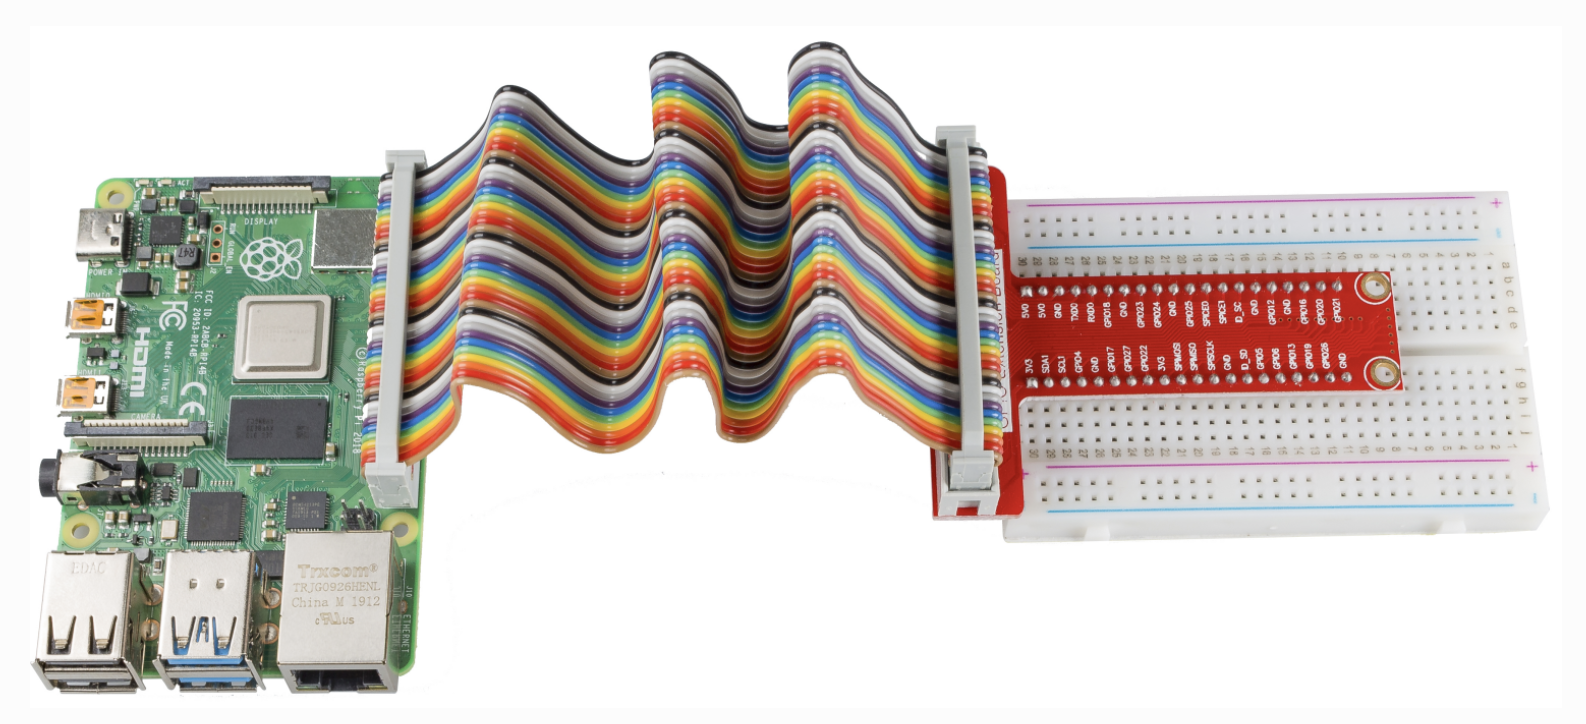
\includegraphics[scale=0.55]{Figs/gpio.png}    
    \end{center}
    \caption{A GPIO extension board \cite{gpio}}
    \label{fig:gpio}
\end{figure}

\begin{figure}
    \begin{center}
        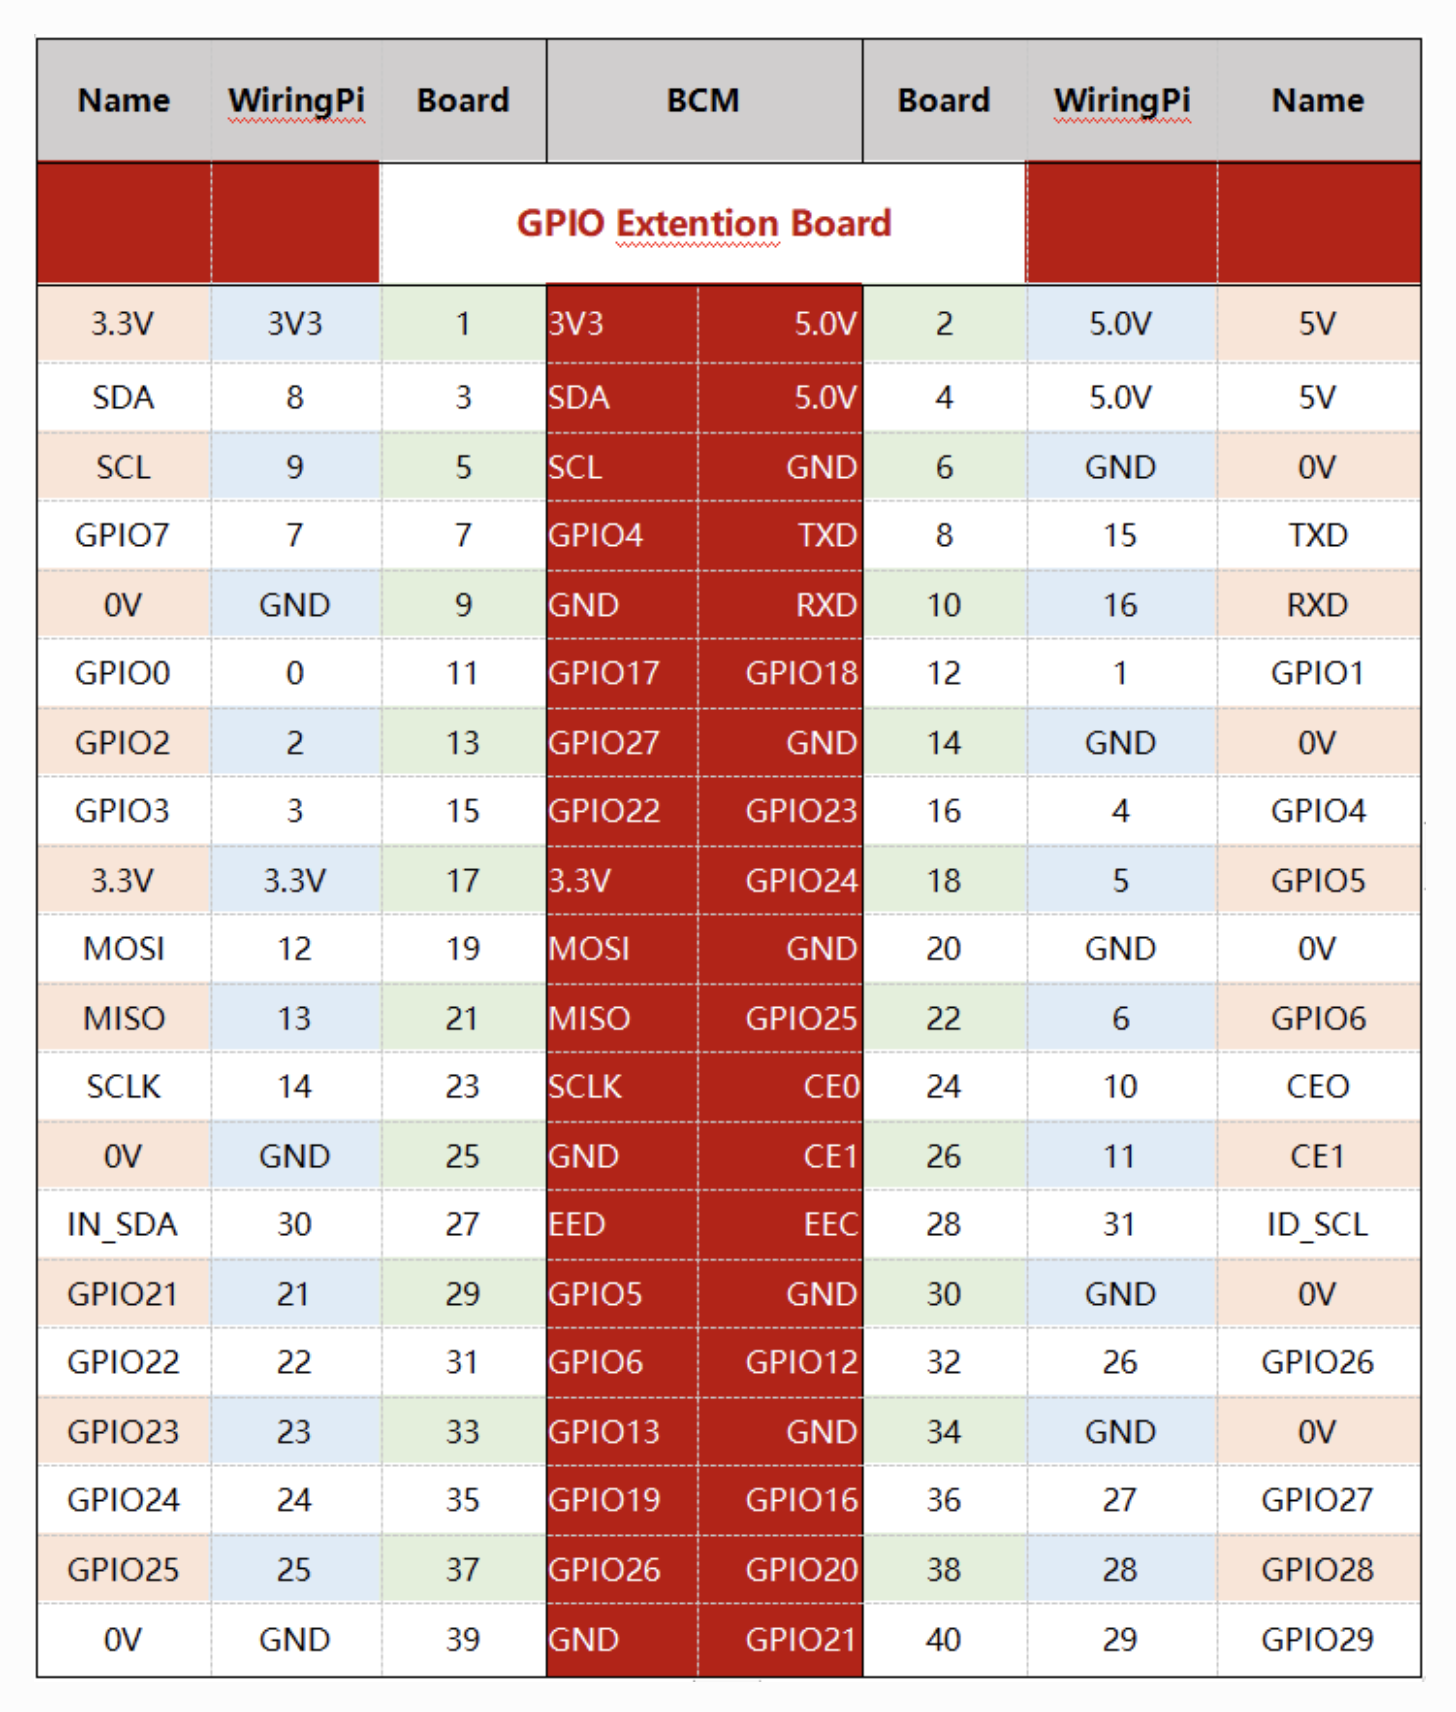
\includegraphics[scale=0.45]{Figs/gpiotable.png}    
    \end{center}
    \caption{Naming methods for WiringPi and Board \cite{gpio}}
    \label{fig:gpiotable}
\end{figure}

\begin{figure}
    \begin{center}
        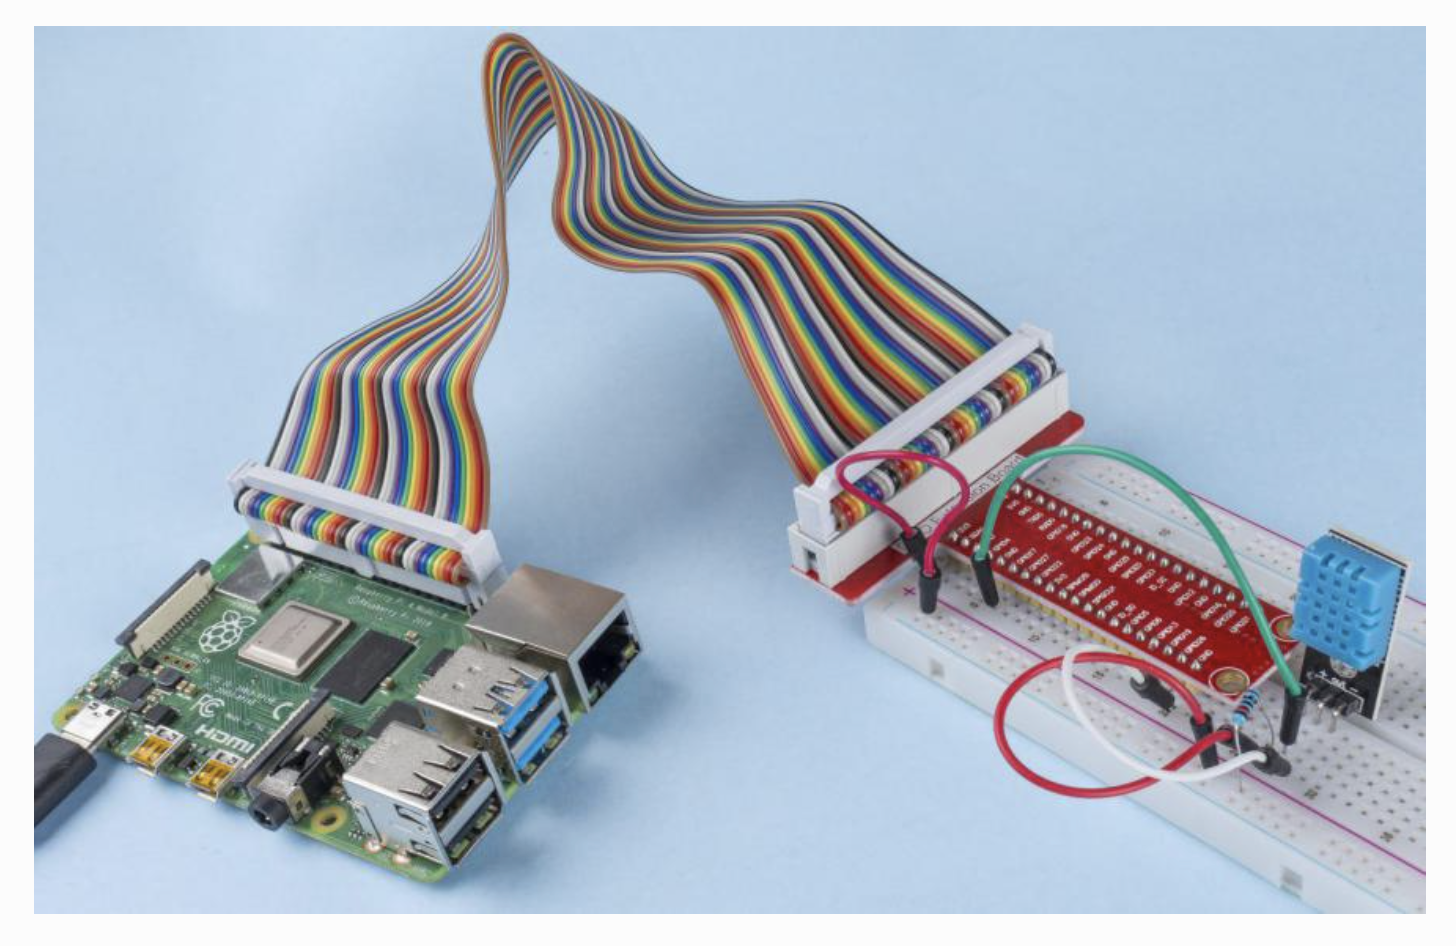
\includegraphics[scale=0.45]{Figs/circuit.png}    
    \end{center}
    \caption{TempSens Hardware Configuration  \cite{circuit}}
    \label{fig:circuit}
\end{figure}

The communication is done over TCP/IP with the help of socket programming. The \texttt{TempSensServer} 
is a bare-bone server which just displays the received information in a proper format. The client collects data for 
one minute before sending the accumulated data to the server. By default, it uses 512 bytes as chunk size. \\
Based off figure \ref{fig:bcm}, the estimated power consumption of wifi adapter is \texttt{1.542} Watts. This 
is calculated after computing the mean average sum of different power modes for different current values 
corresponding to the voltage. In order to compute the optimal chunk size, the python script to determine the 
chunk size was run on the Raspberry Pi 4. \\

\begin{figure}
    \begin{center}
        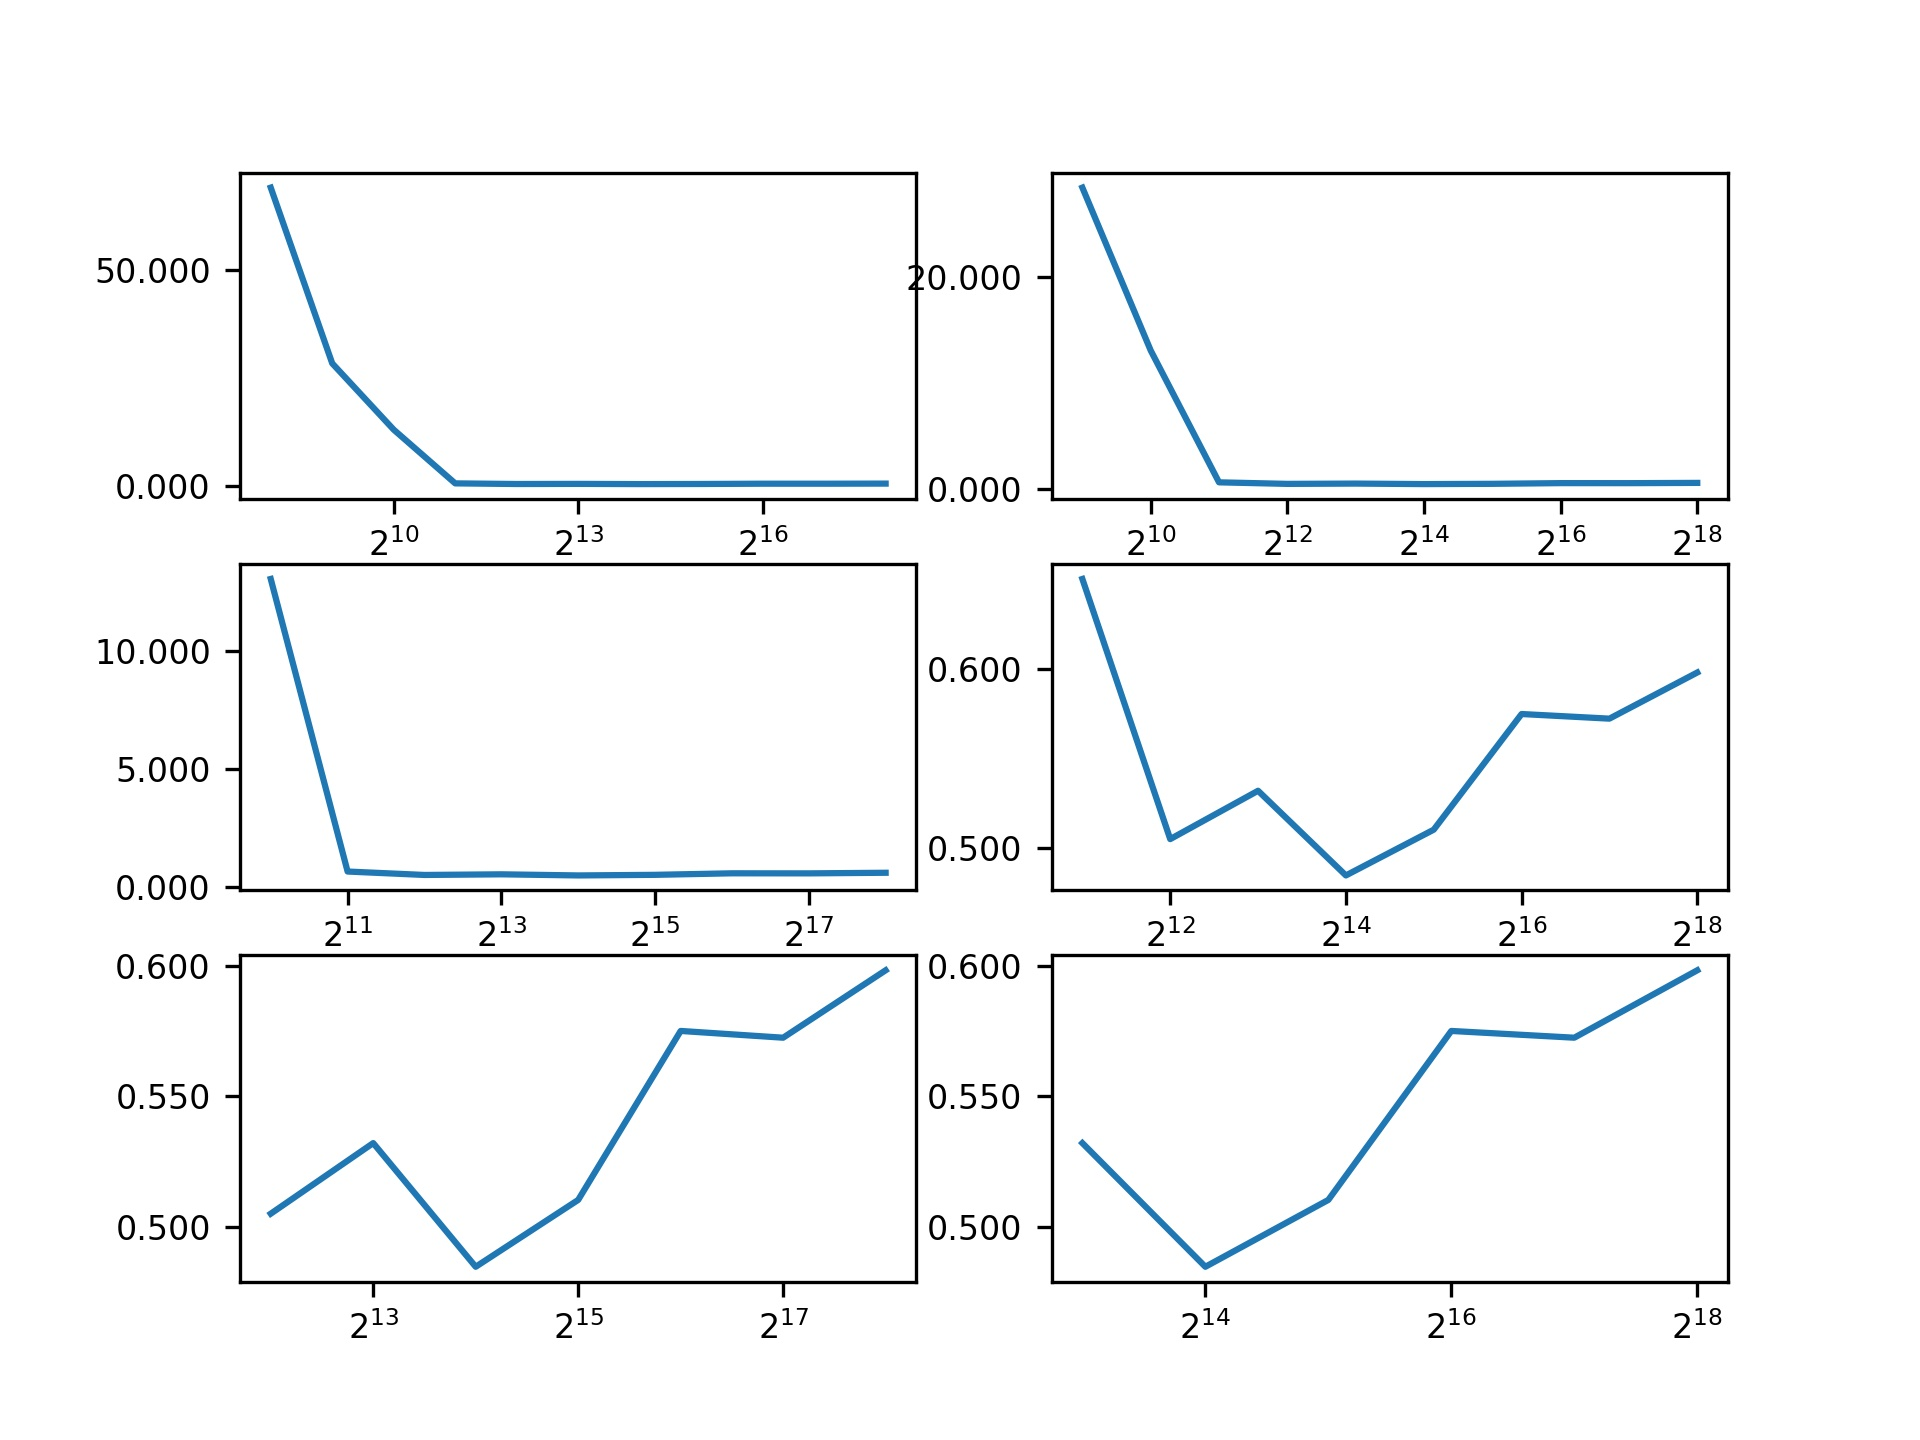
\includegraphics[scale=0.23]{Figs/epbpi.png}    
    \end{center}
    \caption{EPB for different chunk sizes (Chunk Size (x-axis) and Energy in microJ (y-axis))}
    \label{fig:epbpi}
\end{figure}

Figure \ref{fig:epbpi} shows that energy consumption does not linearly depend on chunk size. If that were the case, 
we would have got a straight line. However, what we observe is a global minima and around \texttt{$2^{14}$} on 
the x-axis, we see that's where the lowest amount of energy is being consumed per byte. This suggests that 
for the \texttt{TempSens} app to have optimal energy consumption for communication, the preferred chunk size 
should be \texttt{$2^{14}$} as it would consume the lowest amount of energy. It can also be seen that EPB at \texttt{$2^{14}$} 
is significantly lower than that at the initial value of \texttt{$2^{8}$}. Figure \ref{fig:epbpi} shows multiple 
subplots each for a different range of chunk sizes. The idea behind this is to show that even though the energy 
usage looks pretty much the same when seen in the top-left and top-right plot, but when you actually zoom in 
and see the bottom-left and bottom-right plots, you realize that the energy usage is not that linear anymore. 
There's clearly a global minima present and it will be different for different devices due to varying 
hardware and software configuration but with our work we can definitely find it. \\
Based on the values obtained from this experiment, and then replace them with the default values in \texttt{TempSensClient}, 
the total amount of time for which battery life was prolonged solely due to saving energy in communication cost. 
was about 3 minutes. However, one other use-case of this approach is to be able to determine the intervals at 
which one should communicate data, if it allows. In the case of \texttt{TempSens}, its quite flexible as 
the information being communicated is not time sensitive and the use-case is not that critical. This suggests that 
an optimal interval would be just when the app collects enough amount of data (\texttt{$2^{14}$}). For this app, 
it turned out to be 120 seconds which is double the original interval break. Applying this optimization, we were 
able to prolong the battery time of one charge cycle by 7 minutes. Even though apparently it doesn't sound like much 
but keep in mind this is just with optimizing communication cost which is usually in terms of microJoules. 
Comparatively, that is a considerable improvement in the overall scheme of things. On the other hand, it would 
not have mattered much if the energy usage of the whole device was dependent on a sensor which consumes 
much more energy as compared to the wifi adapter as we will discuss it in the next experimental setup. \\

\section{Experimental Setup \textemdash Fall Detection App}
For this experiment, we test our approach on the Fall Detection App \cite{falld}.

\chapter{Case Study}
% \label{ch:relatedwork}
In this case study, we will discuss how energy consumption is affected if we were to use a containerized environment 
rather than running an application natively. We will also briefly discuss how Lingua Franca, a polyglot coordination 
language for distributed programming, may also contribute towards optimizing energy consumption \textemdash 
albeit for only very specific use cases. 
\section{Docker}
As discussed in Section II, Docker \cite{turnbull_2014} is a container framework which has gained massive 
popularity and real-world application in the past few years. From applications to distributions, one can run 
almost anything inside a containerized environment. Figure \ref{fig:dockerfile} displays a sample 
Dockerfile, which is a script to configure the containerized environment. It can be customized as to one's liking 
and is one of the reasons why Docker has such diverse applications. \\

\begin{figure}
    \begin{center}
        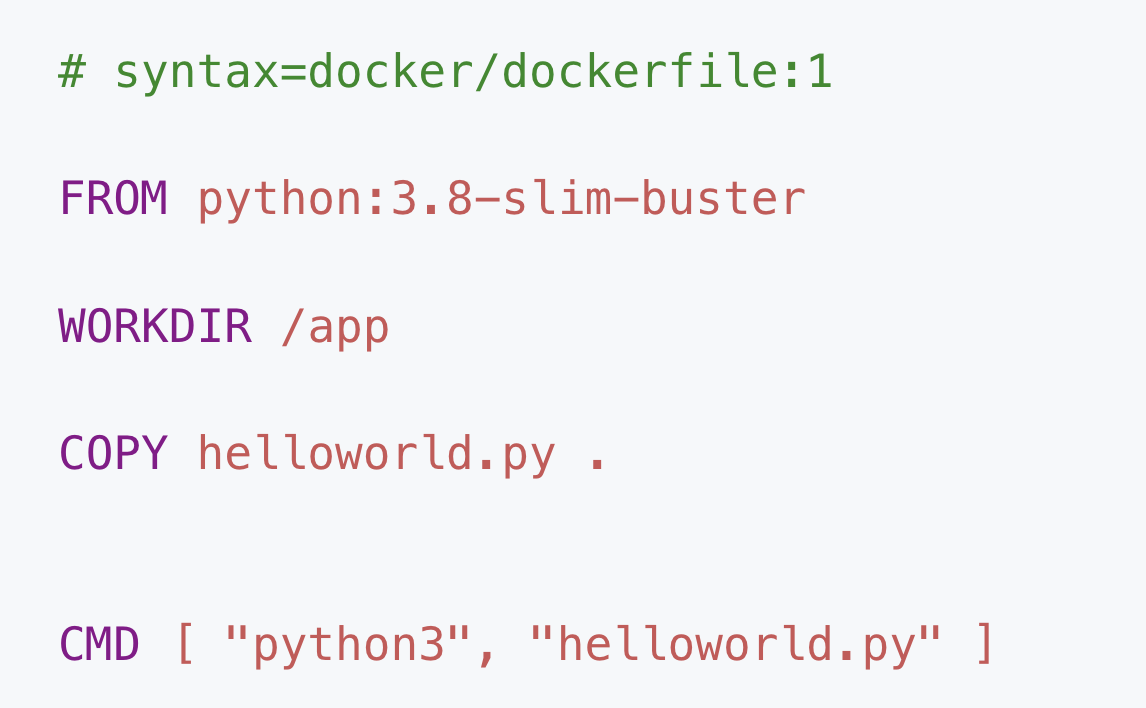
\includegraphics[scale=0.35]{Figs/dockerfile.png}    
    \end{center}
    \caption{A sample Dockerfile}
    \label{fig:dockerfile}
\end{figure}

For this study, we ran \texttt{TempSensClient} as a Docker container on the Raspberry Pi \textemdash we will call 
it \texttt{TempSensClientDocker}. The only thing extra that 
needed to be done was forwarding the port for socket communication when starting up the container. This is due to the 
fact that Docker abstracts the networking layer so the container ports are different from the host ports. The 
assumption for this study was that \texttt{TempSensClientDocker} would consume more energy than \texttt{TempSensClient}. 
However, since we are more interested in communication cost and the energy associated with it, we wanted to 
compare the communication cost. Figure \ref{fig:dockerenergy} shows the EPB for \texttt{TempSensClientDocker} w.r.t 
each chunk size. \\

\begin{figure}
    \begin{center}
        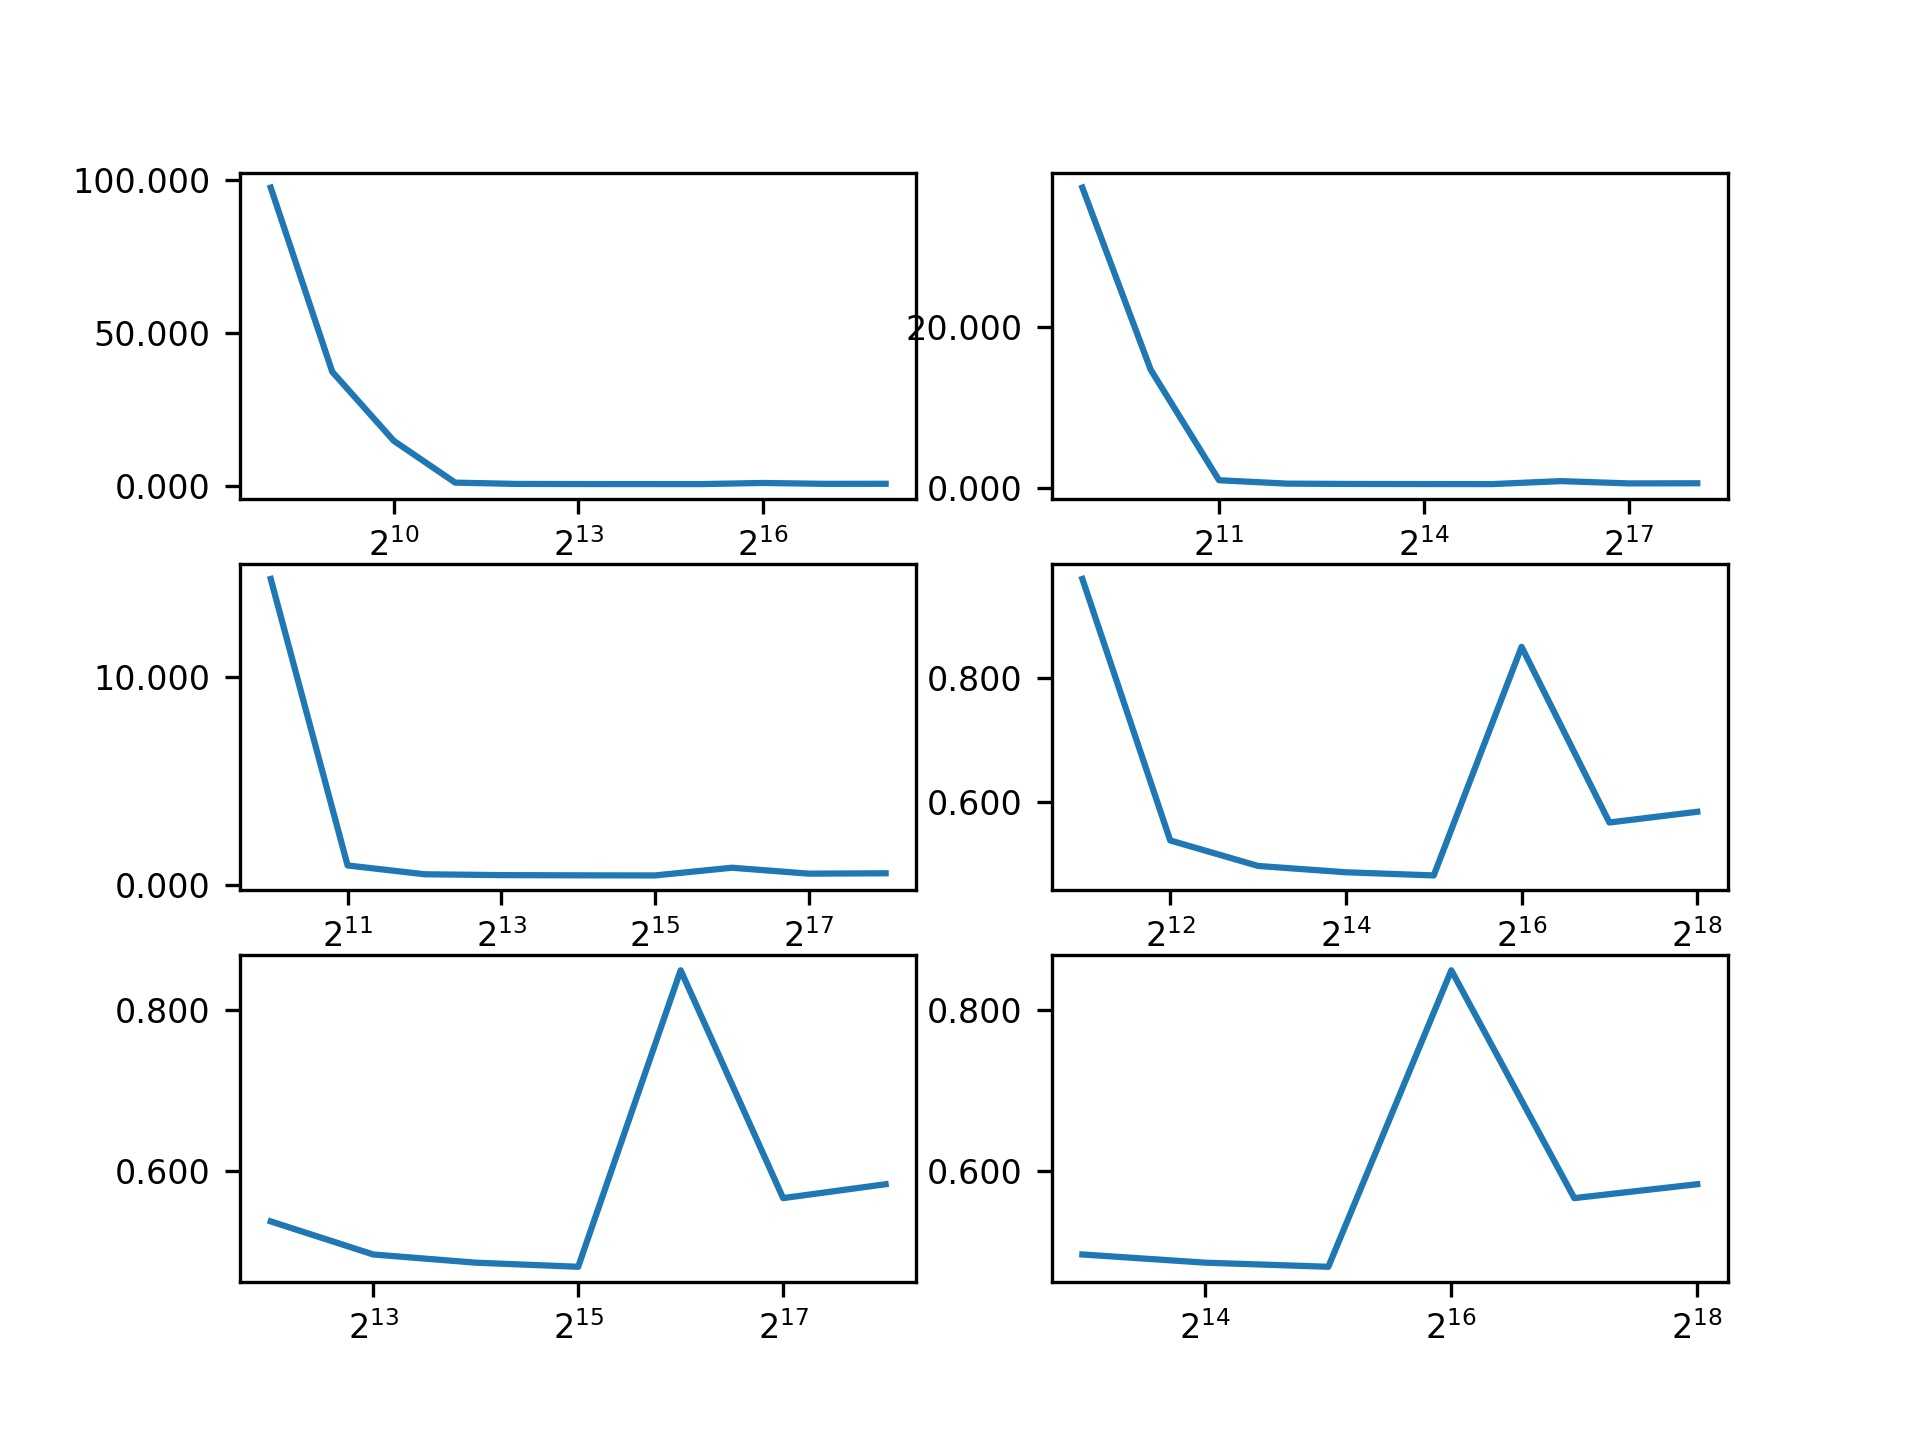
\includegraphics[scale=0.23]{Figs/dockerenergy.png}    
    \end{center}
    \caption{EPB for different chunk sizes (Chunk Size (x-axis) and Energy in microJ (y-axis)) - Raspberry Pi 4 (Docker)}
    \label{fig:dockerenergy}
\end{figure}

This experiment shows that the optimal chunk size for \texttt{TempSensClientDocker} is $2^{15}$ unlike \texttt{TempSensClient} 
that had an optimal chunk size of $2^{14}$. Even though we did expect a little difference between the energy 
consumption, what we did not anticipate was getting a completely different optimal chunk size for the same size on 
the same hardware configuration. Running an application adds an overhead in terms of energy consumption but on the 
other hand provides more maintainability and process isolation. However, the different optimal chunk size is not 
a result of that. As we discussed before, Docker abstracts the networking layer (among other things such as the file 
system) and in order for \texttt{TempSensClientDocker} to be able to communicate with \texttt{TempSensServer} over 
WiFi, we needed to forward the port that the application is supposed to listen at. Recall that in order to compute 
energy consumption, we need both power and time. The power factor here is static and the same as \texttt{TempSensClient} 
however, the abstraction and port forwarding adds to the time factor and therefore, \texttt{TempSensClientDocker} takes 
a tiny bit longer to communicate as compared to \texttt{TempSensClient}, and therefore, has a different optimal chunk size. \\

One question that we would like to ask is that would it be viable to use Docker to achieve energy efficiency? From 
our experiment, it is clear that the optimal chunk size is different and the energy consumption corresponding 
to that is higher than \texttt{TempSensClient} as well. We believe that for the sake of running a single application 
in containerized environment, it is not worth the trade to consume more energy as maintaining one application is 
a somewhat easier task. However, if multiple applications are running inside the same container, then we 
could minimize some of the overhead costs and have a trade-off between maintainability and energy consumption 
depending on the use-case. But, the energy consumption while using Docker would still be greater than running the 
application on a bare-metal OS. This is due to the fact that containers are based on virtualization 
and the I/O system calls that interact with the machine as well as abstractions (such as network layer) 
have a specific overhead. This effect is also discussed by Santos et al. \cite{DBLP:journals/corr/abs-1011-0686} and explains why energy consumption 
is different in a container environment. 

\section{Lingua Franca}
Lingua Franca is a framework developed to provide a coordination language for distributed systems. There are a 
lot of things it is capable of but for the sake of this study, we will focus on features that best relate to 
our work. \\
One of the things that was most interesting was how after writing an LF program, the tool produced efficient code 
for the target programming language. Moreover, it introduces the notion of logical and physical time. Logical time 
is instantiated the moment the program is executed with the system clock's value, which is just the physical time 
at that point. However, logical time progresses differently than physical time. Logical time does not advance 
during the execution of the reaction unlike physical time. Which means that all reactions inside a specific reactor 
are instantaneous. In other terms, two reactions can run concurrently as long as proper variable value handling is done. 
Our assumption was that this could mean the code will execute faster (if possible) given the necessary variables 
had their values instantiated at all possible times, or if the wait time was very minimal. This would further 
help in reduced energy consumption if the program took lesser than usual execution time (with the one time overhead 
of writing the LF equivalent and generating the application code). The code below \cite{lfsource} is an example of concurrent 
reactions being run simultaneously and how the second reaction will print the same result but the process 
 is dependant on 
first reaction's output. To put it simply, if \texttt{out} is set before \texttt{out.is\_present} is called in the 
second reaction, it will double the output and print 42. Otherwise, it will just print 42 (from the \texttt{else} condition) since there is no logical 
information available to determine the wait time in this example. This also show-cases how we can improvise and 
avoid non-determinism. But how much of this actually helps when the application in question is sequential 
and pretty straightforward in question? How does the efficient code generation impact code generation? \\

\begin{lstlisting}{language=Python}
    reactor Source {
    output out;
    preamble {=
        import random
    =}

    reaction(startup) -> out {=
        # Set a seed for random number generation based on the current time.
        self.random.seed()
        # Randomly produce an output or not.
        if self.random.choice([0,1]) == 1:
            out.set(21)
    =}
    reaction(startup) -> out {=
        if out.is_present:
            out.set(2 * out.value)
        else:
            out.set(42)
    =}
    }
\end{lstlisting}

We implemented \texttt{TempSens} purely as an LF application with \texttt{TempSensClientLingua} and 
\texttt{TempSensServerLingua}. The EPB results were similar to Figure \ref{fig:epbpi} because the Python 
source code generated by LF from the above versions was about 99\% identical to our original version. This 
is due to the fact that our application was very simple in nature and also had none of the distributed elements 
that LF could take advantage of. However, we implemented a basic matrix multiplication program in Python 
utilizing parallelism via multi-threading, and then created an LF version for it (see Appendix A). The LF generated 
version was 1.742 seconds slower than the original Python program. There are a number of reasons behind this. 
First, LF has its own overhead because it keeps tracks of logical time among other things. Second, multi-threading 
is not possible using Python since it is not a thread-safe language. The only type of parallelism that can be 
obtained is via multi-processing. And to the best of our knowledge, there is no current LF implementation alternative 
to pool and collect data from multiple processes. \\

The motivation behind this study was to determine whether LF generated programs are more energy-efficient or 
not. From our study, we found out that is not the case with sequential programs with no distributed element 
to them. The \texttt{TempSensClientLingua} took more overall time for communication and hence consumed more energy than 
\texttt{TempSensClient} even though the communication cost was comparable. We believe that since it is designed for 
distributed applications, it would be able to generate more efficient code. However, we also believe that 
the communication cost would not be affected by it since it is not a distributed programming construct but 
since the overall program will be potentially more efficient (due to ease of implementation and understanding 
through LF) in terms of energy consumption. \\
We wanted to conduct a study for the Fall Detection application as well but weren't able to do so due to 
technical limitations. If Fall Detection application were to be implemented as a distributed application, 
we believe that the source code generated by LF would be more energy-efficient. This stems from the fact that 
LF programs are highly specific in terms of functionality without the need for any code bloat, and are 
easier to translate distributed concepts into. This results in less ambiguity and redundancy in the generated 
code and therefore, with fewer instructions to process, it would consume less energy than its natively written 
counterpart. \\
We will discuss the technical limitations in detail in the next section where we will conclude our thesis.
\chapter{Conclusion}
% \label{ch:relatedwork}




\let\svaddcontentsline\addcontentsline
\renewcommand\addcontentsline[3]{%
  \edef\qtest{#1}%
  \def\qmatch{lof}%
  \ifx\qmatch\qtest\else%
    \def\qmatch{lot}%
    \ifx\qmatch\qtest\else%
      \svaddcontentsline{#1}{#2}{#3}%
  \fi\fi%
}

% Appendix - remove this if you don't have an appendix
\addtocontents{toc}{\cftpagenumberson{part}}
\chapter*{APPENDIX SECTION}
\addcontentsline{toc}{part}{APPENDIX SECTION}
\label{ch:appendix}

% restarts the count of figures and tables
\renewcommand{\thetable}{A.\arabic{table}}  
\renewcommand{\thefigure}{A.\arabic{figure}}
\setcounter{figure}{0}
\setcounter{table}{0}

\begin{center}
APPENDIX A
\end{center}

\begin{lstlisting}{language=Python}
# Matrix Multiplication -- LF implementation of Python program
target Python;
preamble {=
    import time
    import threading

    def mult(X, Y):
        result = [[0]*100]
        for z in range(len(Y[0])):
            for k in range(len(Y)):
                result[0][z] += X[0] * Y[k][z]
=}
reactor Source{
    output matrices;
    reaction(startup) -> matrices{=
        m = 100
        X = [[1]*m]*m
        Y = [[1]*m]*m
        matrices.set((X, Y))
    =}
}
reactor Mult{
    input m;
    state threads({=list()=})
    reaction(m){=
        X, Y = m.value[0], m.value[1]
        start = time.perf_counter()
        for i in range(len(X[0])):
            mult(X[i], Y)
        end = time.perf_counter()

        print(f"Time: {round(end - start, 5)} seconds")

        start = time.perf_counter()
        for i in range(len(X[0])):
\end{lstlisting}
\begin{lstlisting}{language=Python}
            x = threading.Thread(target = mult, args=(X[i], Y))
            self.threads.append(x)
            x.start()
        end = time.perf_counter()

        print(f"Time: {round(end - start, 5)} seconds")
    =}
}
main reactor LinguaMatMult{
    src = new Source()
    multi = new Mult()
    src.matrices -> multi.m

}

\end{lstlisting}


%********************************************************************
% Other Stuff in the Back
%*******************************************************
\singlespacing
%********************************************************************
% Bibliography
%*******************************************************
\phantomsection 
\refstepcounter{dummy}
\addcontentsline{toc}{part}{REFERENCES}
\bibliographystyle{ieeetr}
\bibliography{./Bib/References}


% ********************************************************************
% Game Over: Restore, Restart, or Quit?
%*******************************************************
\end{document}
% ********************************************************************
